\chapter{Methodology}
\label{chapter:architecture}

\newenvironment{architecture}
{\quote\itshape}
{\endquote}

\begin{architecture}
\end{architecture}

\section{Sources and Origins of the Dataset}
Constructing a dataset that covers all possible scenarios presents a significant challenge. However, it is feasible to create a comprehensive dataset by including images that represent factors that complicate detection, such as low lighting conditions and poor image resolution. 

The comprehensive exploration and analysis of various online datasets, like COCO \cite{rfc16} and CAVIAR \cite{rfc30}, played a key role in the development of an advanced and realistic dataset, aiming to mirror real-life scenarios, thereby enhancing its applicability in practical contexts. To this end, the dataset integrates images derived from a mock attack scenario \cite{rfc45}, simulating real-world environments like corridors and an entrance area in a university setting. These images, captured from three surveillance cameras, showcase individuals wielding weapons and other scenarios. 

\begin{figure}[h]
    \centering

    % Image 1
    \begin{minipage}{0.47\textwidth}
        \centering
        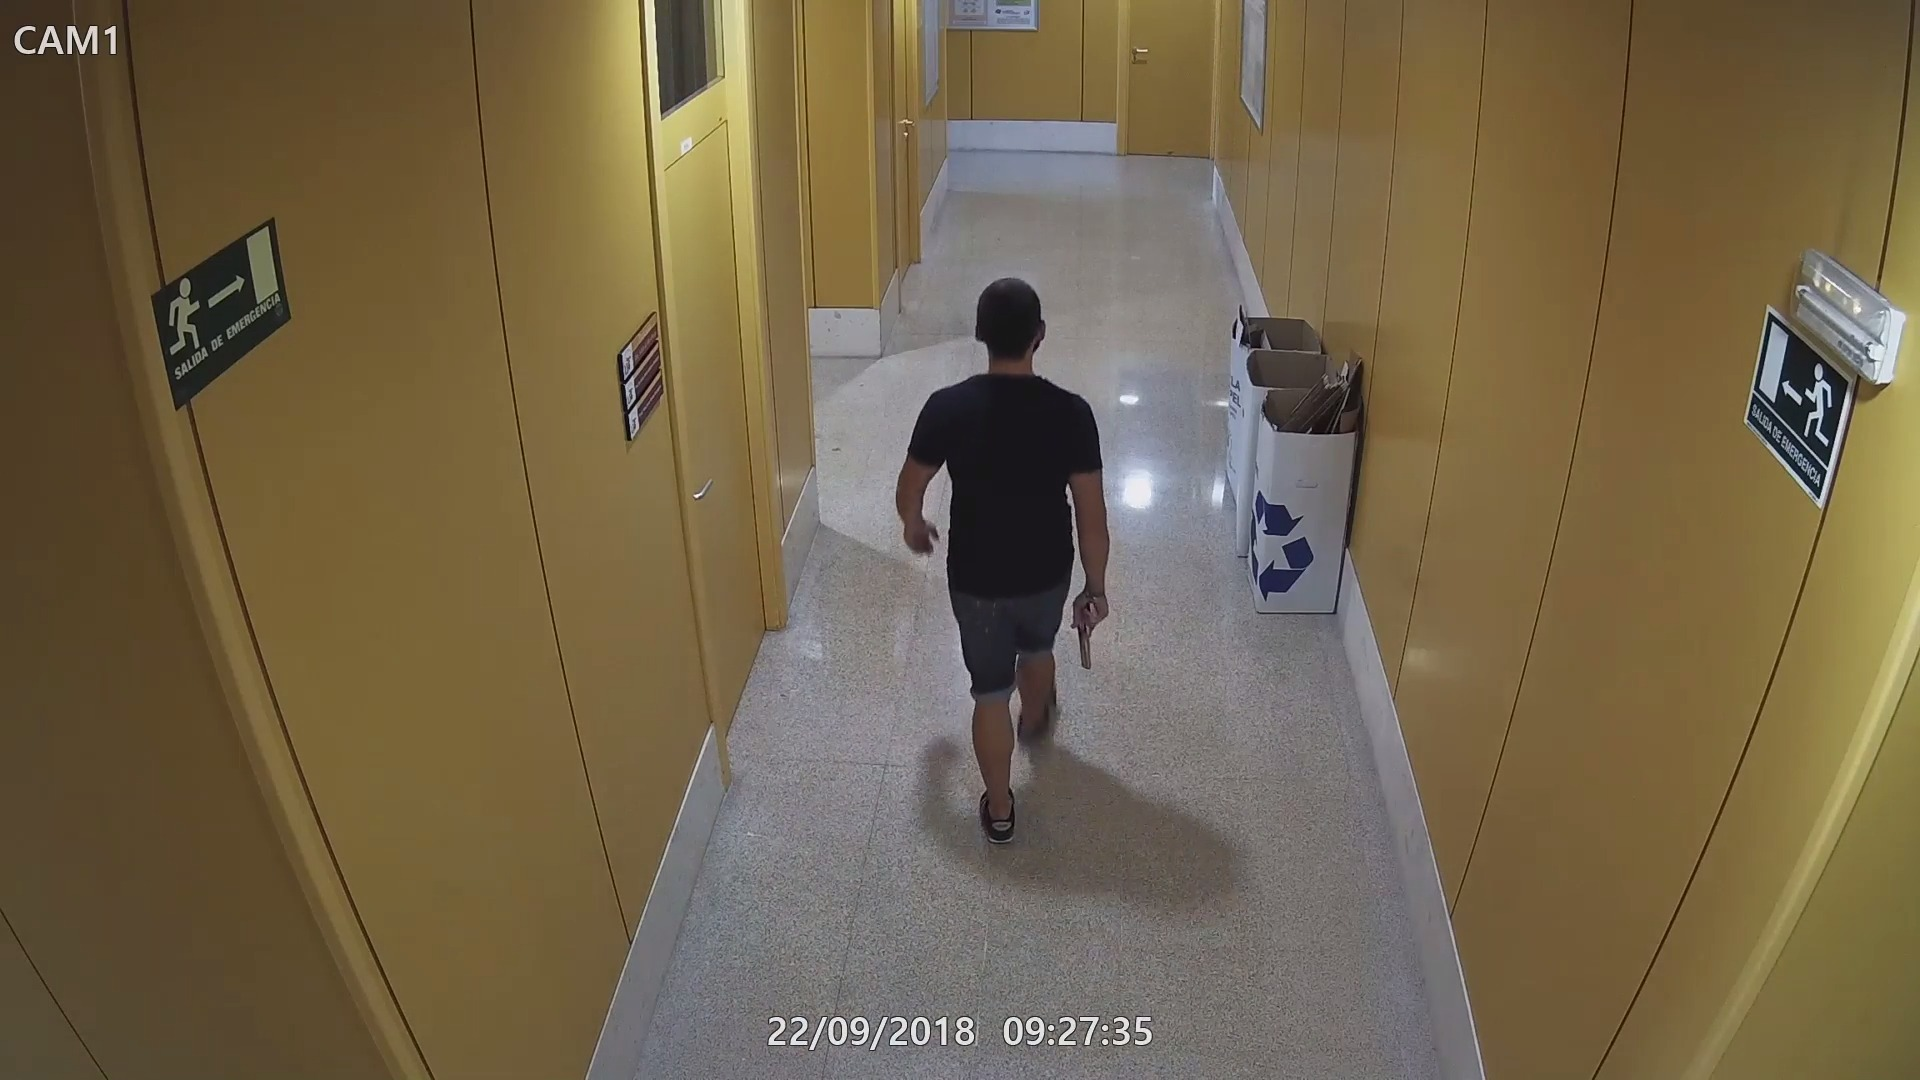
\includegraphics[width=\textwidth]{figs/cam1.jpg} % Include the image
        \caption{Mock Attack Dataset\cite{rfc45} Cam 1 frame}
        \label{fig:cam1}
    \end{minipage}
    \hfill
    % Image 2
    \begin{minipage}{0.47\textwidth}
        \centering
        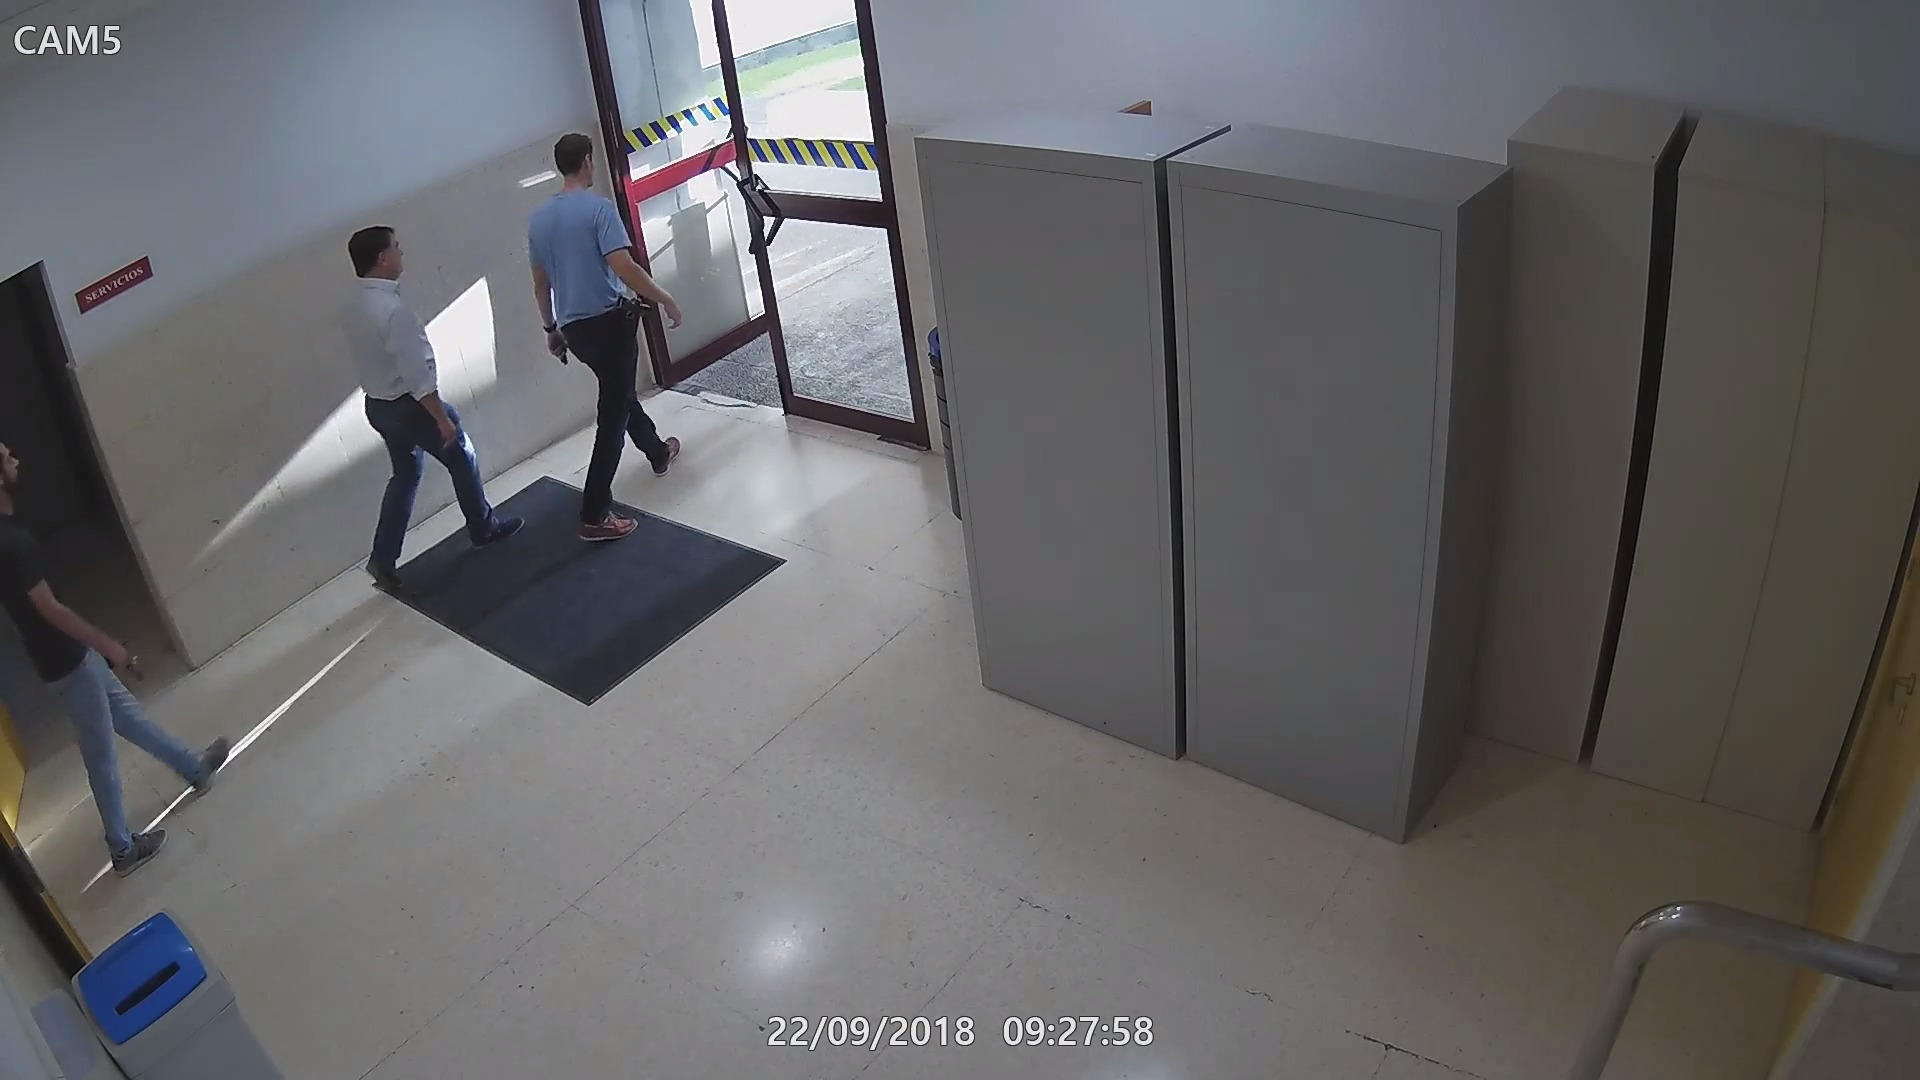
\includegraphics[width=\textwidth]{figs/cam5.jpg} % Include the image
        \caption{Mock Attack Dataset\cite{rfc45} Cam 5 frame}
        \label{fig:cam5}
    \end{minipage}

\end{figure}

The cameras, strategically placed in two different corridors and one entrance, provide a variety of angles and positions, resulting in a rich and diverse visual dataset. Camera 1, in a corridor, recorded 607 frames amidst uniform lighting and obstructions like doors, Figure \ref{fig:cam1}. Camera 7, also in a corridor, gathered 3511 frames, with more complex environments including fire extinguishers. Camera 5, at the entrance, Figure \ref{fig:cam5}, added 1031 frames, distinguished by irregular lighting and obstacles like a black carpet. Annotated at 2 frames per second, these images from different perspectives provide a diverse and realistic depiction of the simulated scenarios.

Additionally, the dataset incorporates a selection of more general images of exposed weapons from the DaSCI collection \cite{rfc29}. This inclusion broadens the scope of the dataset, providing a more comprehensive view of weapon imagery. It also includes images that diverge from the theme of weapons and knives, featuring everyday objects such as wallets or bicycles.

In total, the dataset comprises 11020 images. A strategic division of these images allocates 80\% for training purposes. This portion is crucial for the development and refinement of the object detection model, allowing for extensive learning and adaptation based on a wide array of visual inputs. The remaining 20\% of the images are used for testing. 

Table \ref{datasets-table} presents a dataset summary, listing the source, number of images, resolution, format, and a brief description.
\begin{table}[ht]
    \centering
    \begin{tabularx}{\textwidth}{|l|l|l|l|X|}
    \hline
    \textbf{Source} & \textbf{Images} & \textbf{Resolution} & \textbf{Format} & \textbf{Description} \\ \hline
    \multirow{2}{*}{DaSCI \cite{rfc29}} & 5371 & * & .jpg & Variety of weapons displayed in different positions \\ \cline{2-5}
        & 500 & * & .jpg & Random everyday objects \\ \hline

    \multirow{3}{*}{\centering Mock Attack Dataset \cite{rfc45}} & 607 & 1920x1080 & .png & 
    Cam1: located in one of two corridors, with uniform lighting and some conflicting objects such as doors or bins. \\ \cline{2-5}
     & 3511 & 1920x1080 & .png & 
    Cam5: at the entrance of a university module, features objects like a black carpet on the floor, with irregular lighting. \\ \cline{2-5}
     & 1031 & 1920x1080 & .png & 
    Cam7: in the other corridor, similar to Cam1 but with more conflicting objects. \\ \hline
    \end{tabularx}
    \caption{Summary of Image Datasets and Their Characteristics}
    \label{datasets-table}
\end{table}

\section{High Level Architecture}
Figure \ref{fig:architecture-proposal} illustrates the proposed architecture for the system designed to automatically detect weapons. This system not only identifies weapons but also notifies relevant authorities upon detection. 

\begin{figure}[ht]
    \centering 
    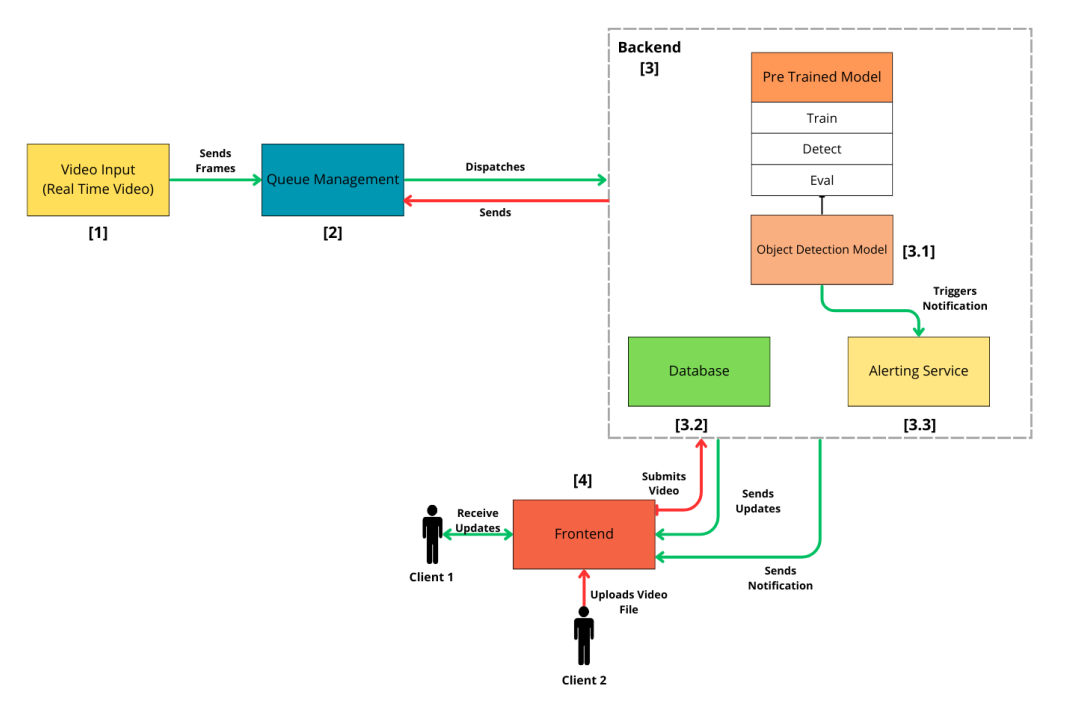
\includegraphics[width=0.95\textwidth]{figs/architecture2.png} 
    \caption{High Level Architecture Proposal}
    \label{fig:architecture-proposal}
\end{figure}

The Video Input (Real-Time Video) [1] consisting of \ac{cctv} cameras strategically installed across various locations, serves as the primary source of video data. These cameras are engineered to capture and transmit real-time video footage, which is then relayed frame by frame to the system for subsequent processing.

The Queue Management component [2] plays a key role in regulating the incoming data flow. It is specifically tasked with receiving video frames from the \ac{cctv} cameras and systematically queuing them for processing. This component is crucial for several reasons:
\begin{itemize}
    \item Load Balancing: effectively manages the influx of video frames, particularly crucial during periods of high input. Without this system, the backend could become overwhelmed, potentially leading to delays or processing failures.
    \item Prioritization: allows for the prioritization of certain video frames or streams, especially those from high-risk areas, ensuring they are processed earlier.
    \item Scalability: as the system expands to accommodate more video sources, Queue Management enables efficient scaling without necessitating significant modifications to the backend processing infrastructure.
\end{itemize}

The backend [3] serves as the system's central processing unit, encompassing a variety of integral modules:
\begin{itemize}
    \item Object Detection Model [3.1]: designed to identify objects of interest, primarily focusing on potentially dangerous items like firearms and knives. It operates with a pre-trained model, which has been finely tuned to pinpoint threats with precision.
    \item Database [3.2]: central to the system's functionality, the database is utilized for storing a wide range of critical data. This includes video metadata, logs of detected objects, model-related data, and other pertinent information that supports the system's operational integrity.
    \item Alerting Service [3.3]: key component of the system, playing a crucial role in ensuring safety. Upon detection of a hazardous object, it promptly generates notifications/alerts. These alerts are then swiftly relayed to the frontend, thereby enabling law enforcement officials to receive real-time updates and respond accordingly.
\end{itemize}

The frontend [4] constitutes a web interface, acting as the primary point of interaction for users, specifically law enforcement officers. It is possible to upload video files directly through the frontend for subsequent analysis. Moreover, it serves as a dynamic platform for receiving timely updates and alerts regarding any detected objects, thereby streamlining the communication process and enhancing the efficiency of law enforcement responses.

\section{Dataset-Model Preliminary Results}
A script was specifically developed to automate the parameter selection for YOLOv5, an advanced deep learning model for object detection. This script not only simplified the model's configuration process but also generated multiple metrics for each test, providing a comprehensive assessment of the model's performance under various parameter settings.

The generated YOLOv5 was then utilized to train and test on the dataset created before with images from Mock Attack Dataset \cite{rfc45}. The model demonstrated an accuracy of 0.9 and, as shown in the F1-confidence curve \ref{fig:f1-score}, achieved an F1 score of 0.87 at a confidence threshold of 0.247. This was achieved following 100 training epochs and using a batch size of 64.

\begin{figure}[h]
    \centering 
    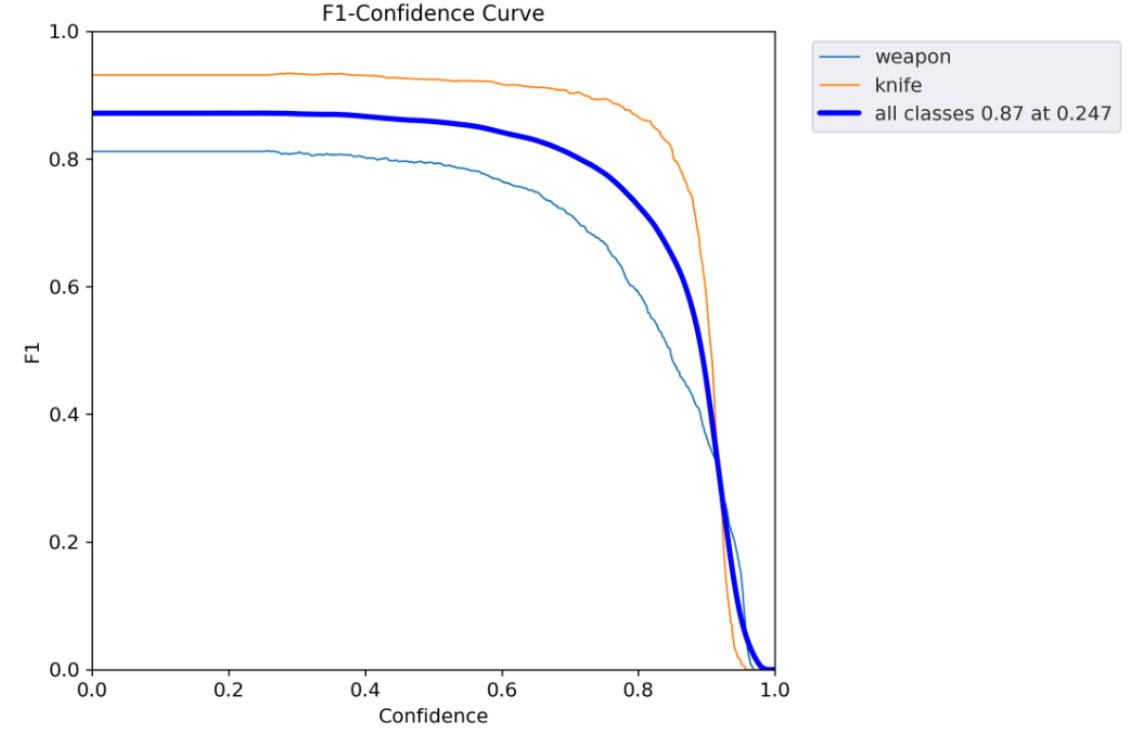
\includegraphics[width=0.65\textwidth]{figs/f1-score.png} % Include the image
        \caption{F1-score results with 100 epochs and using a batch size of 64}
        \label{fig:f1-score}
\end{figure}

\section{Work Plan and Milestones}
The thesis's work plan is presented in the Gantt chart (Figure \ref{fig:gantt}), which maps out the timeline for each task to the development process. This chart illustrates a strategic methodology, guaranteeing a methodical and efficient advancement of the project. 

The efficiency of the project results from the implementation of a bottom-up\footnote{approach where the development process begins with the smallest or most basic elements, gradually integrating these into a comprehensive system or structure} approach. This method, reflecting the architectural design strategy previously mentioned, is crucial for success. It facilitates the iterative building of a system that is both robust and scalable.

In parallel, the thesis writing progresses in an iterative manner alongside the development tasks. This simultaneous documentation approach ensures the continuous incorporation of new insights and findings into the thesis. This strategy not only enriches the content but also guarantees that the documentation aligns with the ongoing development.

\begin{figure}[H]
    \centering
    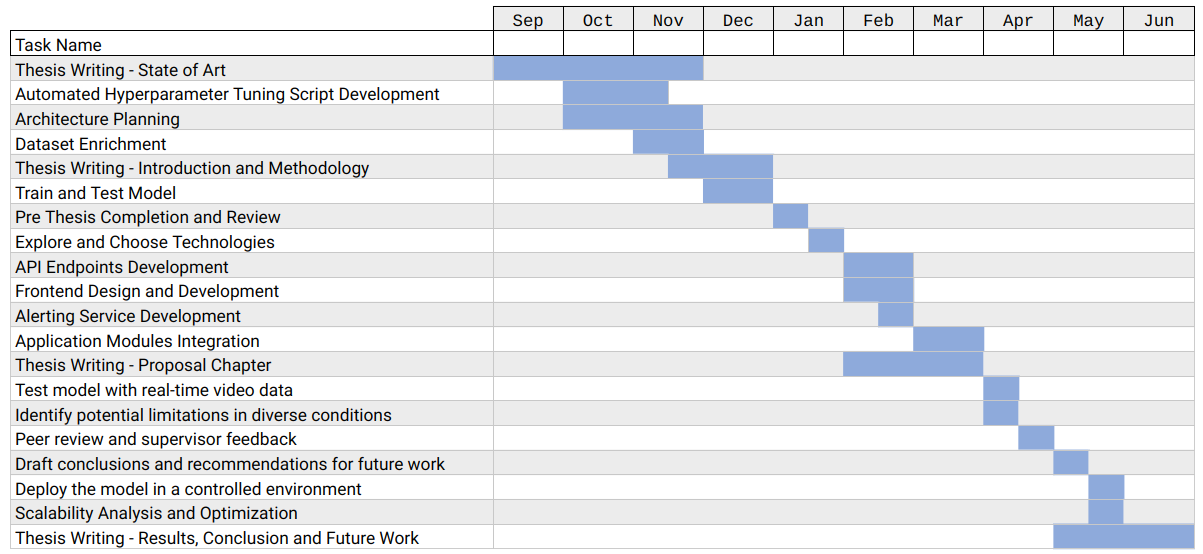
\includegraphics[width=0.9\textheight, height=0.6\textwidth, keepaspectratio, angle=90]{figs/gantt.png}
    \caption{Gantt Chart Timeline for Project Management and Development Stages}
    \label{fig:gantt}
\end{figure}
